62. \begin{figure}[ht!]
\center{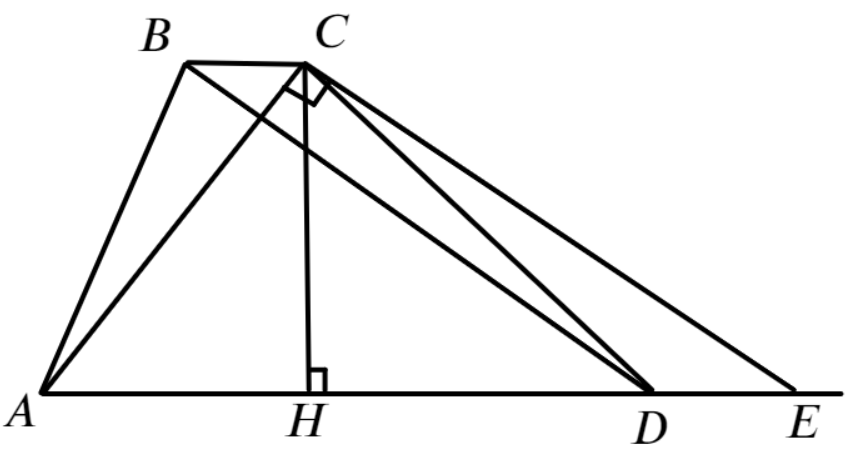
\includegraphics[scale=0.35]{g9-61.png}}
\end{figure}\\
Пусть диагональ $BD=5.$ Проведём через вершину $C$ прямую, параллельную $BD,$ точку её пересечения с прямой $AD$ обозначим буквой $E.$ Тогда $BCED$ является параллелограммом, а значит $CE=BD=5$ и $BC=DE,$ а значит $AE=AD+DE=AD+BC=2\cdot6,5=13.$ Так как $AC\perp BD,$ то и $AC\perp CE.$
Опустим высоту $CH,$ тогда $S_{ABCD}=\cfrac{1}{2} CH\cdot (AD+BC)=\cfrac{1}{2} CH\cdot AE=S_{\Delta ACE}.$ Найдём $AC=\sqrt{13^2-5^2}=12,$ тогда $S_{\Delta ACE}=\cfrac{12\cdot5}{2}=30.$\\
